\section{Introduction}\label{sec:intro}

Speculative decoding lets a small drafter propose several tokens that the target model verifies in a single forward pass \citep{leviathan2023fast,chen2023accelerating}. Its benefit depends on how many proposals the target accepts, and a drafter trained offline loses acceptance when the traffic differs from its training data. Several systems therefore keep adapting the drafter while it serves, using the target's own outputs as supervision \citep{liu2024osd,qian2026drafts,wang2026aurora,park2026tide}. On our code workload, a factory EAGLE-3 drafter for Qwen3-8B raises its acceptance length from \nv{lc.code.n0} to \nv{lc.code.n3200} after learning online from 3{,}200 requests.

A better drafter does not by itself make serving faster. Figure~\ref{fig:motivation} shows three effects that a serving system has to weigh (\cref{sec:measure}). First, whether speculation pays at all depends on load and architecture: for Qwen3-8B with short outputs, speculation is \nv{sweep.short.c1}\% faster than plain decoding with one request in flight but \nv{sweep.short.c256abs}\% slower with 256, whereas on the Qwen3-30B-A3B mixture-of-experts (MoE) target it is still \nv{sweep.moe.c256}\% faster with 256. Second, training on the serving GPU is not free: a trainer running a fraction $d$ of the time removes roughly $d/2$ of the serving throughput. Third, drafters reach very different ceilings: the Chinese drafter covers only \nv{cover.zh}\% of the target's output tokens with its draft vocabulary and stalls at acceptance \nv{lc.zh.n3200}, far below the \nv{astar.zh.c256} it would need to beat plain decoding at saturation, and the function-calling drafter peaks after \nv{lc.fc.peakN} requests and then declines.

These effects couple the two decisions a serving system has to make, whether to use the drafter and whether to improve it. Training helps only if the improved drafter will be used, which depends on the load; and at saturation, using the drafter may become worthwhile only after training. Sharing the GPU between training and serving is attractive, because online adaptation needs little compute: in our runs the controller trained on at most about \nv{full.tok.max} million tokens per run, so a dedicated training GPU, as used by Aurora and TIDE, would sit idle most of the time. Sharing also means that every second of wasted training, for example on a drafter that can never reach break-even, is a second of lost serving.

We build a controller for this co-located setting (\cref{sec:method}). Every second it decides whether to speculate, how much of the GPU the trainer may use, and when the trainer should export a new drafter or stop. It relies on a calibration made once per model and domain before deployment: a profitability frontier, the break-even acceptance length as a function of concurrency, and a learning curve. Speculation is enabled only above break-even. Training uses the latency slack below the service-level objective (SLO) when there is slack; under saturation it runs only if the gain predicted over a forecast horizon repays the throughput it costs; and it stops when the reachable acceptance cannot cross break-even, when the drafter is at its ceiling, or when a new drafter no longer raises acceptance. We implement the controller in vLLM \citep{kwon2023vllm} with a live feature export from the serving path, hot replacement of the drafter, and a runtime speculation switch (\cref{sec:system}), and port it to SGLang (\cref{sec:sglang}).

We evaluate with every component frozen in one checkpoint (\cref{sec:evaluation}): \nv{n.runs} paired runs over three scenarios (Qwen3-8B code, Qwen3-8B Chinese, Qwen3-30B-A3B code), \nv{n.pol} policies, and three repetitions. The best fixed policy differs by scenario: plain decoding for Chinese, and a training schedule that is told when to stop for the two code scenarios. Every other policy falls at least \nv{alt.minshort}\% short of the per-scenario best in some scenario; the controller stays within \nv{full.worstshort}\% in all three. 
We further evaluate the controller in a frozen simulator using unseen workload traces and randomized drift scenarios, with pre-declared criteria for goodput, training efficiency, and workload robustness (\cref{sec:heldout}).

Our contributions are:
\begin{itemize}
\item A measurement study of how speculation, co-located training, and online adaptation interact on a dense and an MoE target, including where a better drafter cannot pay off (\cref{sec:measure}).
\item A controller that couples a calibrated profitability frontier with learning curves to decide when to speculate, how much to train, and when to stop, implemented in vLLM with live feature export, drafter hot replacement, and a runtime speculation switch, and ported to SGLang (\cref{sec:method,sec:system,sec:sglang}).
\item A frozen-checkpoint evaluation with paired repetitions against \nv{n.pol} policies, including an informed schedule and an acceptance-triggered policy in the style of TIDE, and a frozen-simulator validation on unseen traces with pre-declared criteria, reported together with the claims it weakens (\cref{sec:evaluation}).
\end{itemize}

\begin{figure*}[t]
\centering
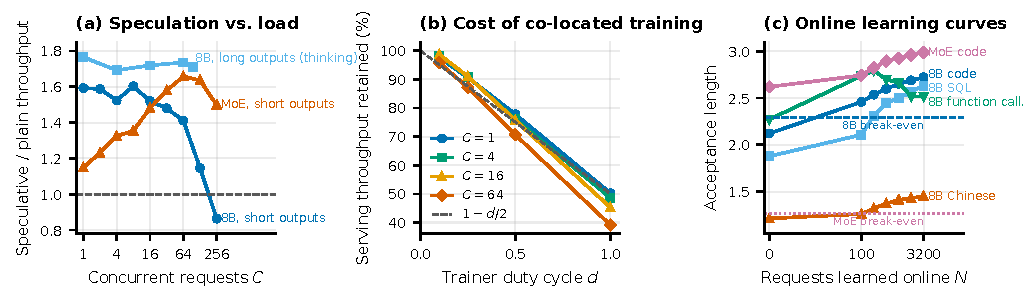
\includegraphics[width=\linewidth]{figures/fig1_motivation.pdf}
\caption{Calibration measurements (one H100, vLLM 0.27.1, factory EAGLE-3 drafters, $k{=}3$). (a) Speculative over plain-decoding throughput versus concurrency. (b) Serving throughput retained when a trainer shares the GPU at duty cycle $d$ (Qwen3-8B, short outputs, speculation on); the dashed line is $1-d/2$. (c) Acceptance length after learning online from $N$ requests; dashed lines mark the break-even acceptance at $C{=}256$ (Qwen3-8B code: \nv{astar.code.c256}; MoE code: \nv{astar.moe.c256}).}
\label{fig:motivation}
\end{figure*}
